\documentclass[12pt,a4paper]{article}

% Paquetes esenciales para LuaLaTeX
\usepackage{fontspec} % Manejo nativo de fuentes en LuaLaTeX (reemplaza a inputenc)
\usepackage[spanish, es-tabla]{babel}
\usepackage{graphicx}
\usepackage{geometry}
\usepackage{hyperref}
\usepackage{xcolor}
\usepackage{listings}
\usepackage{booktabs}
\usepackage{tabularx}

% Configuración de márgenes
\geometry{
    top=2.5cm,
    bottom=2.5cm,
    left=3cm,
    right=3cm
}

% Configuración para bloques de código Java
\definecolor{codegreen}{rgb}{0,0.6,0}
\definecolor{codegray}{rgb}{0.5,0.5,0.5}
\definecolor{codepurple}{rgb}{0.58,0,0.82}
\definecolor{backcolour}{rgb}{0.95,0.95,0.92}

\lstdefinestyle{javastyle}{
    backgroundcolor=\color{backcolour},   
    commentstyle=\color{codegreen},
    keywordstyle=\color{blue},
    numberstyle=\tiny\color{codegray},
    stringstyle=\color{codepurple},
    basicstyle=\ttfamily\footnotesize,
    breakatwhitespace=false,         
    breaklines=true,                 
    captionpos=b,                    
    keepspaces=true,                 
    numbers=left,                    
    numbersep=5pt,                  
    showspaces=false,                
    showstringspaces=false,
    showtabs=false,                  
    tabsize=2
}
\lstset{style=javastyle}

\begin{document}

% Portada
\begin{titlepage}
    \centering
    
    % ESPACIO PARA EL LOGO
    
    {\scshape\LARGE Universidad de las Américas Puebla \par}
    \vspace{0.5cm}
    {\scshape\Large Departamento de Computación, Electrónica y Mecatrónica\par}
    \vspace{2cm}
    
\includegraphics[width=0.45\textwidth]{img/logo_udlap.jpg} % Reemplaza con el nombre de tu archivo de imagen
    \vspace{1.5cm}

    {\huge\bfseries Proyecto - F1 \par}
    \vspace{0.5cm}
    {\Large FORMULA CHEMS\par}
    \vspace{0.5cm}
    {\large Programación Orientada a Objetos (POO)\par}
    \vspace{2.5cm}
    
    {\Large Presentado por:\par}
    \vspace{0.5cm}
    {\large Amy Marianee Ramírez Sánchez \par}
    {\large Juan Pablo López Moreno \par}
    {\large Jose Maria Blancarte López \par}
    
    \vfill
    {\large \today \par}
\end{titlepage}

\newpage
\tableofcontents
\newpage

\section{Contexto}
Llamada la competencia por excelencia del automovilismo, la Fórmula 1 (F1) es una serie de carreras que impulsan al límite la tecnología, la ciencia y las construcciones que participan en ella. 

Esta competencia está compuesta por una variedad de elementos, entre los cuales se encuentran temporadas de carreras denominadas "Gran Premio", la culminación de 3 clasificatorias y más de 2 docenas de pilotos compitiendo por los mejores tiempos.

\section{Motivación}
La Fórmula 1 es el deporte de autos más popular del mundo, donde cada segundo cuenta y se genera una cantidad enorme de datos en cada carrera. Lo que nos motiva a desarrollar este proyecto es el reto de tomar toda esa información (equipos, pilotos, tiempos y resultados) y ordenarla en un sistema fácil de usar. 

Queremos diseñar una herramienta sencilla que limpie la complejidad de los datos, permitiendo a cualquier aficionado entender los resultados y revivir la emoción de cualquier temporada de forma clara.

\section{Objetivos}
Desarrollar un sistema orientado a objetos para registrar y administrar la información de las temporadas de Fórmula 1, con la capacidad de almacenar de forma independiente y reproducir el historial estadístico de cualquier año de competición.

\subsection*{Objetivos específicos:}
\begin{itemize}
    \item \textbf{Administrar escuderías y recursos técnicos:} Orquestar la creación de equipos deportivos aplicando restricciones reglamentarias estrictas (límites operativos de pilotos), y parametrizar las características mecánicas de los monoplazas (motor, llantas y peso en escalas validadas) junto con el factor de habilidad de cada conductor.
    
    \item \textbf{Calendarizar y configurar Grandes Premios:} Estructurar la temporada de competición definiendo el nombre, nivel de dificultad y las ventanas de tiempos históricos (mínimos y máximos) para cada circuito, permitiendo el control del progreso cronológico del año.
    
    \item \textbf{Registrar clasificaciones mediante simulación probabilística:} Procesar los tiempos de las sesiones Q1, Q2 y Q3 utilizando funciones de distribución gaussiana para modelar estadísticamente la variabilidad de la pista, y aplicar un motor lógico de filtrado que asigne posiciones iterativamente hasta ensamblar la parrilla de salida oficial.
    
    \item \textbf{Controlar resultados y campeonatos globales:} Simular la carrera dominical ponderando la habilidad del conductor, la eficiencia del vehículo y factores de aleatoriedad para el cálculo de rebases, documentando las posiciones finales y actualizando automáticamente el estado del campeonato mundial.
    
    \item \textbf{Generar reportes visuales y persistencia de datos:} Producir de forma automatizada tablas gráficas e indicadores de desempeño accesibles para el usuario, asegurando la trazabilidad de la simulación mediante la exportación y lectura estructurada de archivos en formato JSON.
\end{itemize}

\section{Enfoque}
Basándose en esta necesidad y en la pasión compartida por un deporte tan tecnológicamente complejo, avanzado e innovador. El proyecto se centra en responder una pregunta clave: ¿Es posible administrar y recrear los resultados de la Fórmula 1 usando el paradigma de programación orientada a objetos?

Siguiendo esta pregunta, y convencidos de sus posibles soluciones, presentamos este documento como reporte de las propuestas, desarrollos e implementaciones de esta solución.

\section{Fase de Análisis}
Debido a las particulares necesidades del problema consideramos este flujo básico para poder cumplir con las relaciones. Lo que se busca con las relaciones establecidas en el flujo es permitirnos adaptar a cualquier cantidad de escuderías y pilotos por cada temporada.

\begin{figure}[h!]
    \centering
    % ESPACIO PARA LA IMAGEN DEL GRAFO F1
    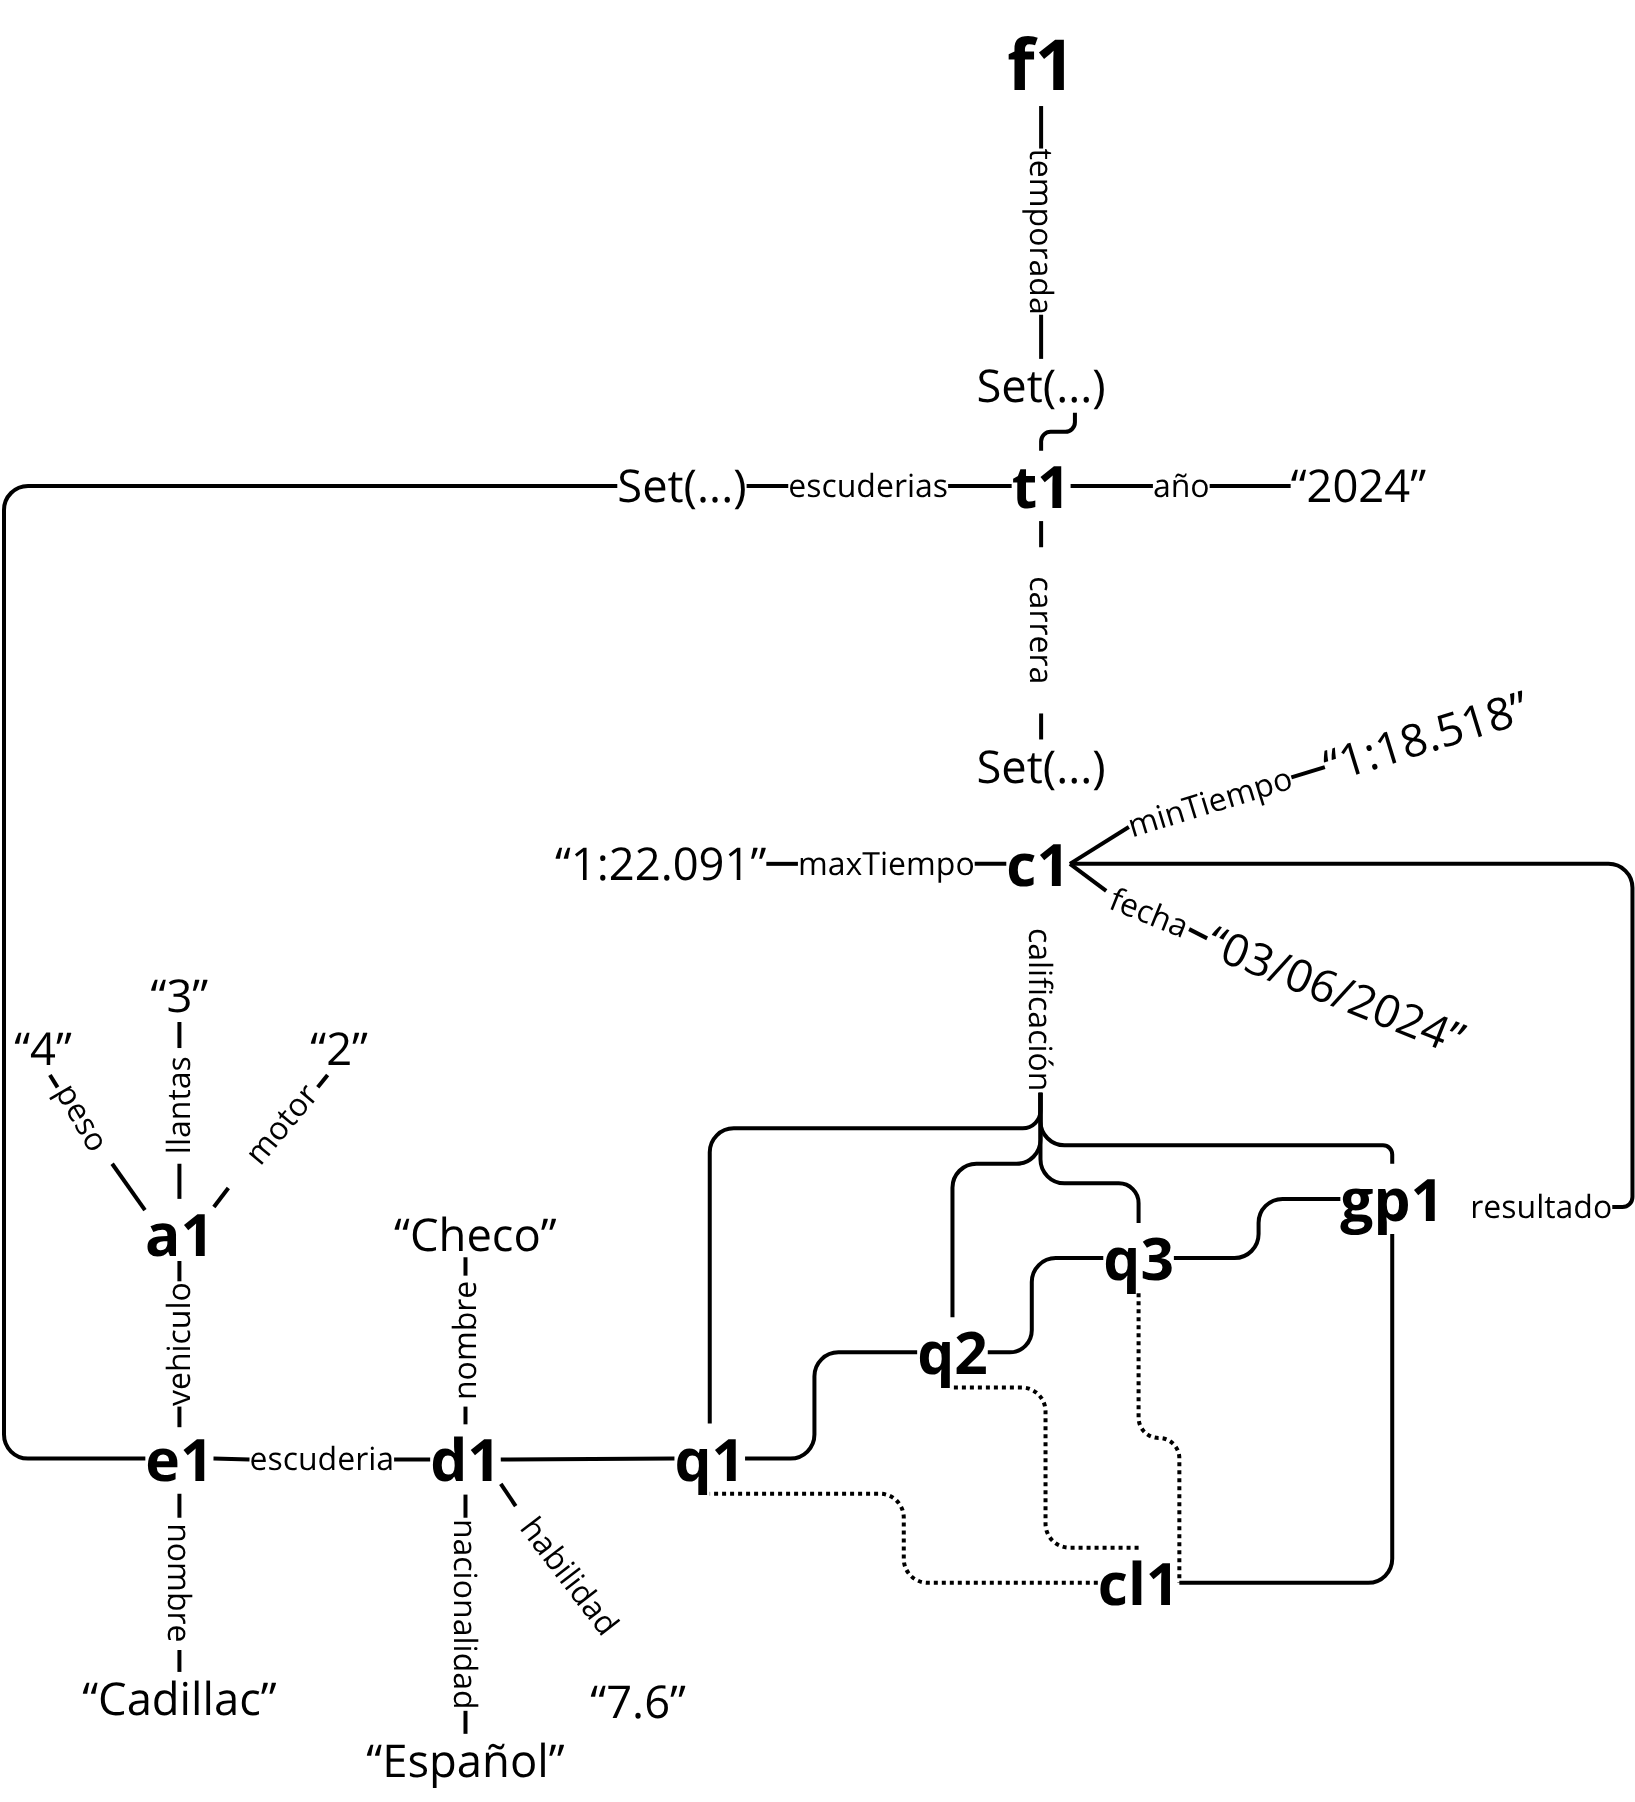
\includegraphics[width=0.8\textwidth]{img/grafo_f1.png}
    \caption{Diagrama de relaciones lógicas F1}
\end{figure}

Las relaciones entre los objetos se establecieron siguiendo un flujo de dependencias lógicas muy claro: la temporada rige las carreras y las escuderías; las escuderías agrupan los recursos operativos como los vehículos y los pilotos; y las carreras controlan la ejecución de las sesiones competitivas. 

El vehículo y el piloto se diseñaron como entidades separadas pero vinculadas a la escudería, lo que otorga la flexibilidad necesaria para modificar las características de un auto o los datos de un conductor sin alterar la estructura general del equipo. Por otro lado, la bifurcación de la carrera en sesiones de clasificación divididas en etapas y una carrera final permite que los tiempos medidos en las primeras fases sirvan como el criterio de ordenamiento para la parrilla de salida, reflejando fielmente las reglas de la competencia. 

Con este planteamiento, se abarca la gran mayoría de los requerimientos solicitados en esta primera etapa, ya que el modelo es capaz de almacenar con precisión los datos logísticos de los premios, el inventario técnico de los equipos y los resultados de las posiciones alcanzadas tanto en pruebas como en el Gran Premio definitivo. Es fundamental destacar que el diseño actual constituye un avance inicial y una base sólida para el proyecto, enfocado primordialmente en la correcta administración, almacenamiento y consistencia de los datos históricos de la Fórmula 1. Al tener esta estructura de herencia y asociaciones bien definida, el sistema queda completamente preparado para escalar en fases posteriores del desarrollo. 

Más adelante, se planifica trabajar con la implementación de algoritmos avanzados y lógica de programación matemática que aprovechen atributos clave como el nivel de habilidad del piloto, las características de los neumáticos o el rendimiento del motor. Esto permitirá realizar cálculos complejos, simulaciones de carreras en tiempo real basadas en probabilidades y la predicción de resultados competitivos con un nivel de precisión mucho mayor, transformando el sistema de una base de datos estática a un entorno dinámico de simulación deportiva.

\section{Fase de Diseño}
En la fase de diseño el equipo se enfocó en mejorar las propuestas, optimizar el desarrollo y completar todos los objetivos. Al modificar el planteamiento inicial, ampliamos varios métodos y clases para poder implementar de manera ordenada y más orientada a objetos, estableciendo el flujo y relaciones existentes entre las diversas clases. 

El desafío principal de esta sección radica en establecer las relaciones apropiadas para hacer el mayor uso de todos los atributos y clases, sobre todo los vínculos entre las clases como Carrera y sus dependientes como Q1, Q2 y Q3, cuyas clases también tienen un vínculo de dependencia con Clasificación para poder procesar las listas adecuadas. 

Asimismo, establecer un orden apropiado para distribuir y aprovechar ciertos comportamientos tenemos la clase Tabla la cual tiene interacciones con Carrera, Clasificación y Temporada. Todos estos cambios a las bases principales, al igual que las relaciones necesarias para el diseño y posterior implementación fueron reducidas a este diagrama UML (Unified Modeling Language), las cuales señalan todas las características del diseño de la solución.

\begin{figure}[h!]
    \centering
    % ESPACIO PARA LOS DIAGRAMAS UML
    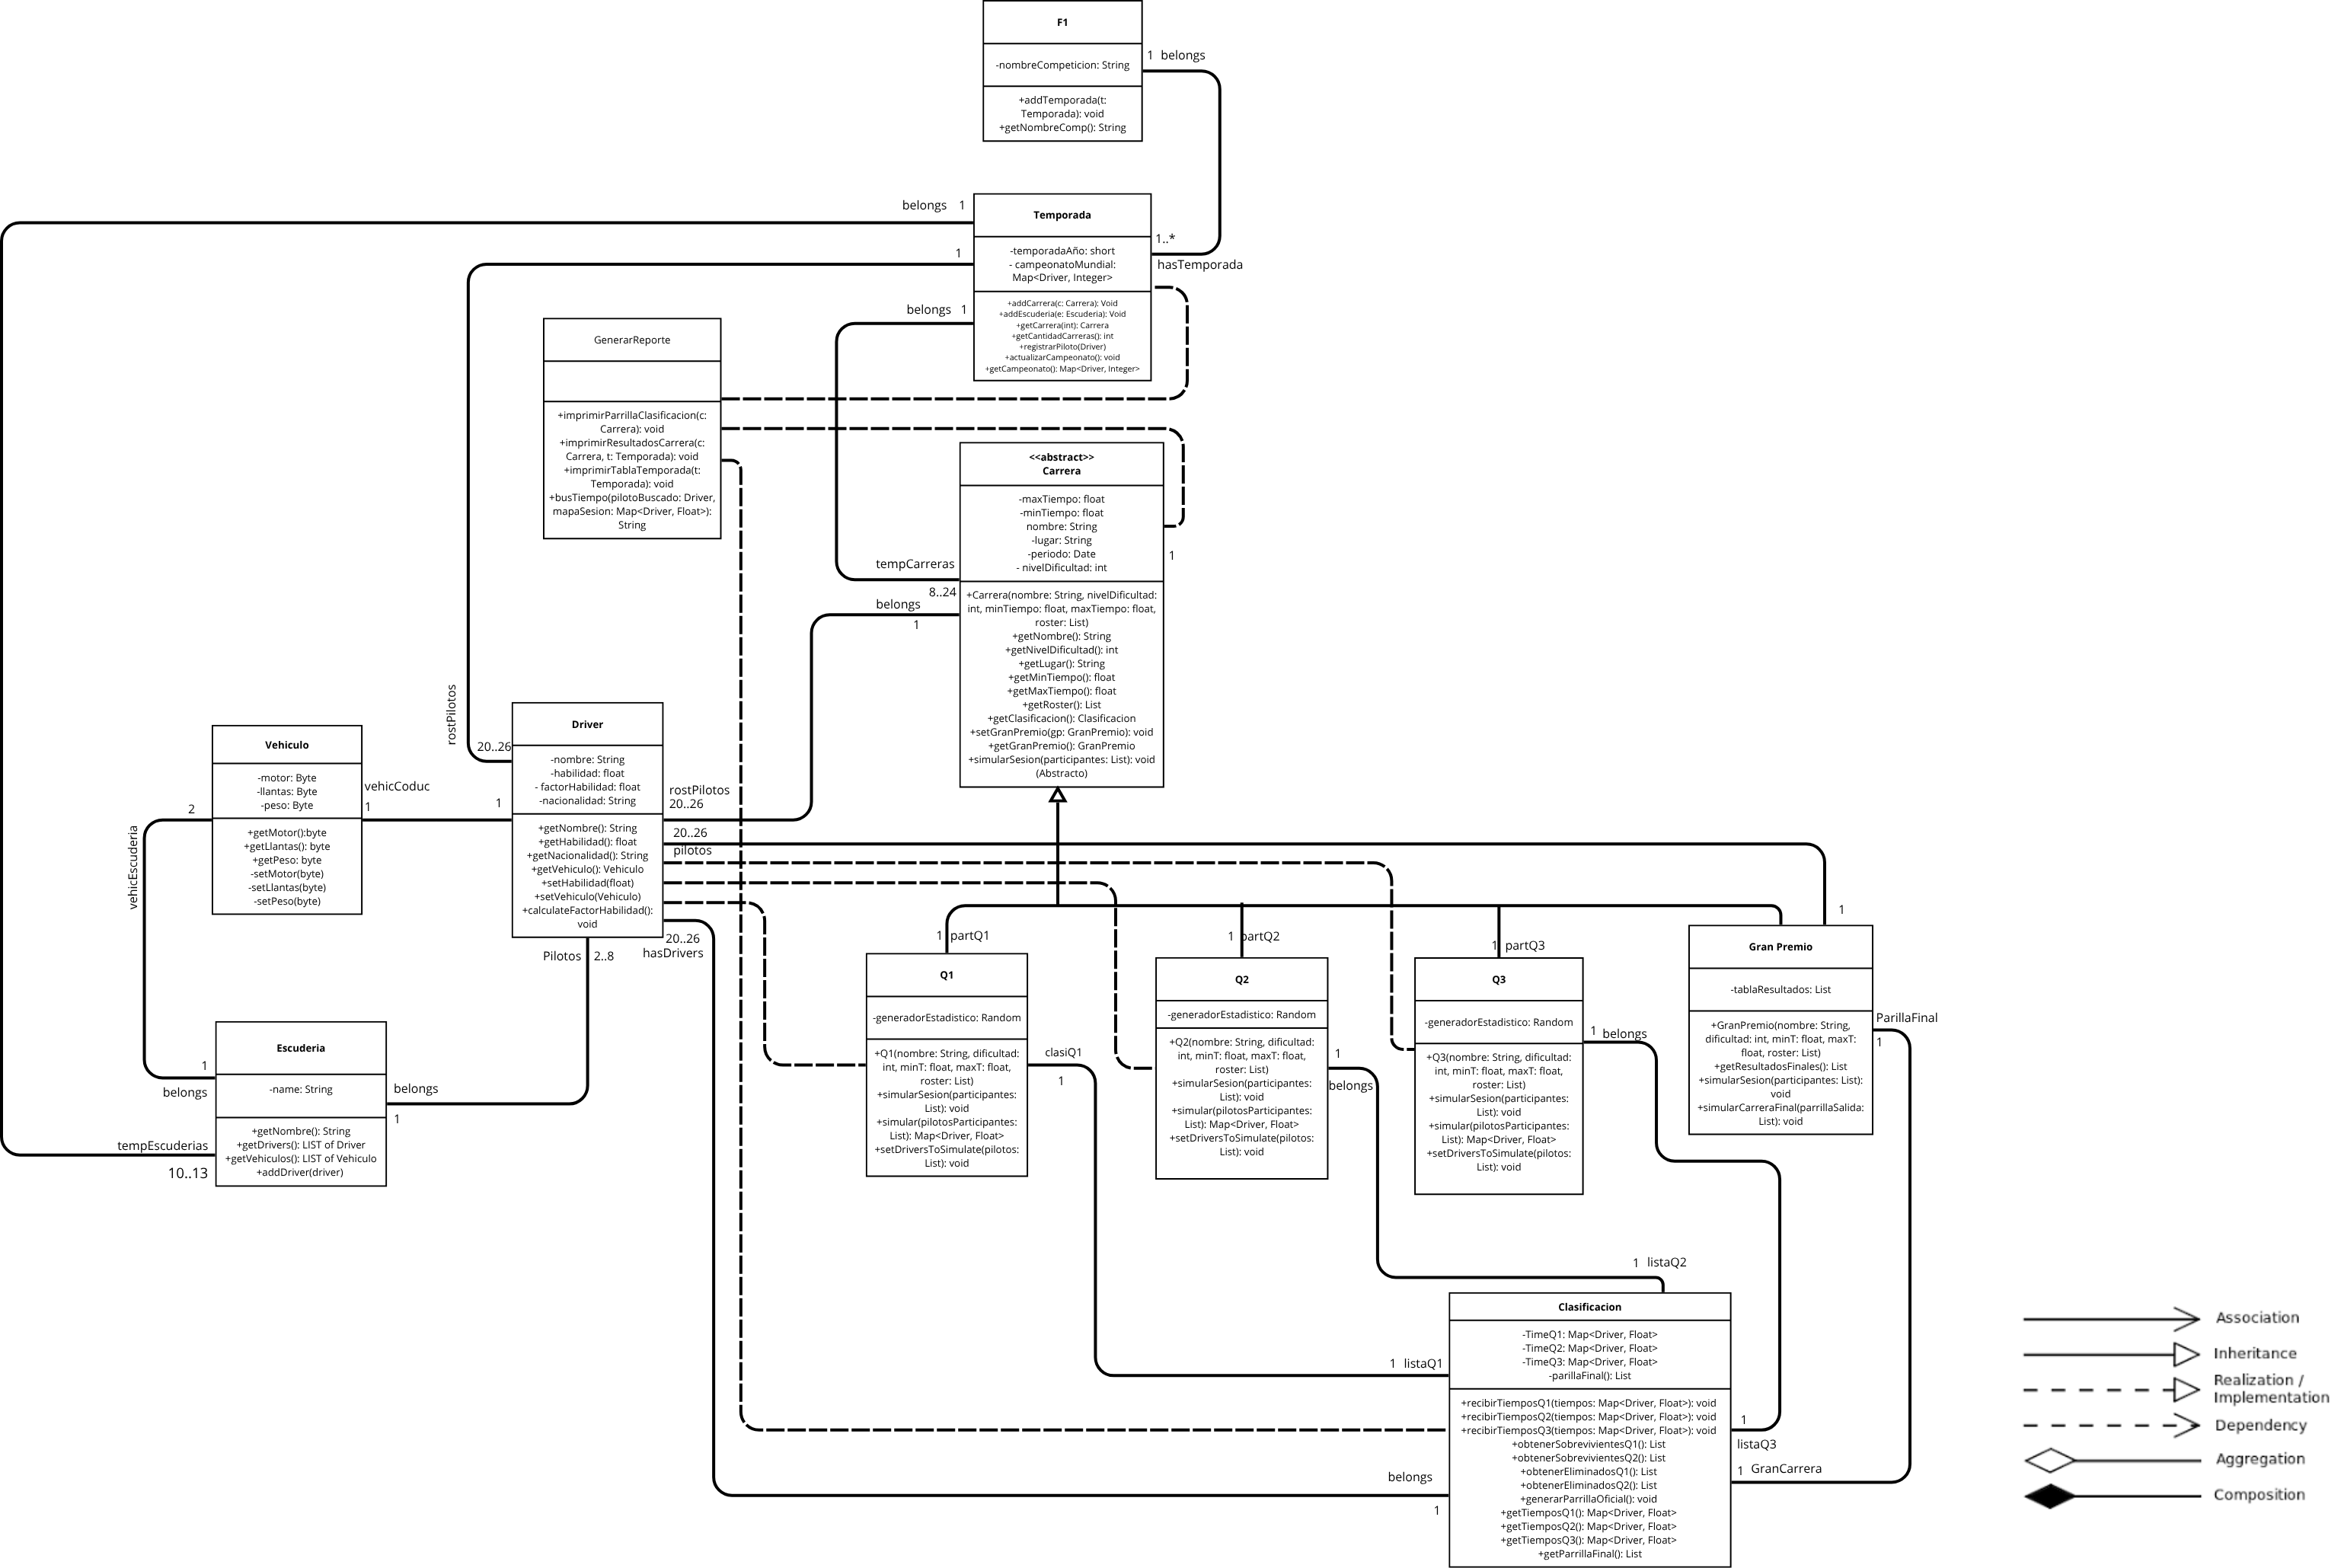
\includegraphics[width=\textwidth]{img/diagrama_uml.png}
    \caption{Diagrama de clases UML}
\end{figure}

\noindent Link para una mejor visualización de los diagramas: \url{https://canva.link/0gsla7v19ifsfgk}

\section{Implementación}
\subsection{Entidades Básicas}
\begin{itemize}
    \item \textbf{Vehículo:} Esta clase nos permite establecer los parámetros básicos de cada vehículo, incluyendo su peso, llantas y motor. Incluye excepciones para evitar valores inadecuados.
    \item \textbf{Driver:} Se desarrolló esta clase para mencionar las características principales de todos los pilotos, incluyendo nombre, nacionalidad y su habilidad (del 0 al 10). Esta clase es primordial para obtener tanto los resultados, como afectar las posibilidades del piloto en las carreras.
    \item \textbf{Escudería:} La implementación de esta clase se realiza con el motivo de agrupar a los pilotos con sus vehículos. Esto nos permite reunir los factores necesarios para influir en los tiempos de la carrera, y forzar a la existencia de únicamente 2 vehículos en cada escudería, junto con mínimo 2 pilotos y máximo 8 pilotos (2 activos y otros 6 de repuesto permitidos por la FIA, 4 pilotos por vehículos).
\end{itemize}

\subsection{Motor de Simulación}
\begin{itemize}
    \item \textbf{Carrera:} La clase de carrera nos ayuda a definir el nombre de la pista, su nivel de dificultad y los tiempos máximos y mínimos históricos (para poder simular los tiempos dentro de esto). Asimismo, esta clase contiene un método abstracto \texttt{simularSesion()} el cual en clases de qualis (Q1, Q2, Q3) se fuerce a simular según se dicte en cada clase.
    \item \textbf{Q1, Q2, Q3:} Estas clases heredan todo de Carrera y ocupan sus propias fórmulas matemáticas para poder realizar el cálculo y lista de los tiempos de los pilotos. El equipo implementó una campana gaussiana para poder determinar la complejidad de cada Qualy, con diferentes factores (1.2, 1 y 0.8) para determinar la desviación estándar de los eventos.
    \item \textbf{Gran Premio:} Simula el evento principal de los domingos, y basado en probabilidades establece mediante la parrilla de inicio los resultados finales de cada carrera. Esto mediante la implementación de un factor de aleatoriedad, que por cada piloto adyacente, se genera un número decimal pseudo aleatorio entre 0.0 y 1.0 usando \texttt{Math.random()}, para después establecer la condición \texttt{Math.random() > 0.75} que instituye a cualquier piloto que caiga dentro de esta condición un intercambio de posición (simulando el rebase). Guardando la lista modificada como tabla de posición final al terminar el recorrido.
\end{itemize}

\subsection{El Flujo y Control de Datos}
\begin{itemize}
    \item \textbf{Clasificación:} Nos ayuda a guardar al piloto con su tiempo y mediante Stream de Java, nos permite establecer quienes pasan al siguiente Qualy, asimismo, nos apoya creando la parrilla a partir de los eliminados y los resultados de todos los clasificatorios.
    \item \textbf{Temporada:} El equipo desarrolló una clase que nos permite analizar el año, escuderías, carreras y puntos recopilados durante cada temporada. Asimismo, nos permite resimular una temporada, borrando la tabla de puntos y simulado desde la carrera 1 de la temporada.
\end{itemize}

\subsection{Director de Orquesta}
\begin{itemize}
    \item \textbf{Main:} En esta clase de prueba configuramos los 22 vehículos y los 22 pilotos con los datos reales de la temporada 2026. Las 11 escuderías existentes y 24 carreras para la temporada. Igual se configuró un switch básico para poder realizar acciones y llamar métodos.
\end{itemize}

\section{Anexos}
\subsection{Justificación SO2}
\begin{itemize}
    \item \textbf{Identify:} El proyecta se enfoca en las vida real, estableciendo las regulaciones y limitaciones de acuerdo a los reglamentos y estándares establecidos por la FIA y las empresas detrás de la carrera. Esto se refleja, por ejemplo, en la clase de \textbf{Escudería}, con las limitantes del numero de pilotos y vahiculos.
    \item \textbf{Analyze:} Para simular una variabilidad estadística se implementó una campana gaussiana con ciertas desviaciones establecidas en cada Qualifier, estos pasados en el comportamento real de las carreras y resultados, basado en los tiempos históricos. 
    \item \textbf{Evaluate solutions:} Un efoque principal del proyecto fue asegurar la comparación y facilidad de acceso a los datos simulador para su comparativa a futuro. 
    \item \textbf{Develop Solutions:} Varios intentos se realizaron para poder realizar de mejor manera las simulaciones y llegar al objetivo final. Por esta misma razón se ocupó el archivo \textbf{\textit{Manejador de Archivos}}, para mejorar el proyecto basado con alternativas tecnológicas.
    \item \textbf{Implement Engineering Design:} El proyecto al implementarse se considera 100\% funcional, escalando su funcionamiento mediante una interfaz gráfica, la lógica se ensambla de manera completa de manera jerarquica.
    \item \textbf{Consider non-techincal issues:} EL proyecto se desarrollo con un enfoque basado en fans de la Fórmula 1, buscando una simplicidad y facilidad de acceso con los usuarios. Considerando todas las posibilidades y aceptando la mejora y desarrollo según las necesidades de los usuarios. 
\end{itemize}

\subsection{Códigos para S02}
\subsubsection{Identify}
\begin{lstlisting}[language=Java, caption={Restricciones y estándares en Vehículo y Escudería}]
// Fragmento de Vehiculo.java demostrando restricciones de ingeniería (0 a 10)
public void setMotor(byte mo) {
    if (mo < 0 || mo > 10) {
        throw new IllegalArgumentException("La caracteristica debe estar entre 0 y 10. Valor intentado: " + mo);
    }
    this.motor = mo;
}

// Fragmento de Escuderia.java demostrando restricciones logísticas
private static final byte MIN_PILOTOS = 2;
private static final byte MAX_PILOTOS = 8;

public Escuderia(String n, Vehiculo v1, Vehiculo v2, List<Driver> drivers){
    if(drivers.size() < MIN_PILOTOS || drivers.size() > MAX_PILOTOS){
        throw new IllegalArgumentException("La lista de pilotos debe tener entre " + MIN_PILOTOS + " y " + MAX_PILOTOS + " para ser valida.");
    }
    this.nombre = n;
    // ...
}
\end{lstlisting}

\subsubsection{Analyze}

\begin{lstlisting}[language=Java, caption={Análisis estadístico en Carrera.java}]
/*
 * Ecuación única centralizada para simular tiempos de clasificación.
 * Utiliza los bonos de habilidad e ingeniería de cada piloto, aplicando la
 * desviación estándar configurada de manera particular por cada subclase.
 */
public Map<Driver, Float> simularFase(List<Driver> pilotosParticipantes) {
    Map<Driver, Float> resultados = new HashMap<>();
    
    for (Driver d : pilotosParticipantes) {
        float bonoHabilidad = d.getHabilidad() * 2.5f;
        float bonoVehiculo = (d.getVehiculo().getMotor() / 10.0f) * 2.5f;
        
        float media = maxTiempo - bonoHabilidad - bonoVehiculo;
        
        // Generación del tiempo usando la desviación de la sesión actual
        float tiempo = media + ((float) rng.nextGaussian() * desviacionEstandar);
        
        if (tiempo < minTiempo) {
            tiempo = minTiempo + (rng.nextFloat() * 0.2f);
        }
        resultados.put(d, tiempo);
    }
    return resultados;
}
\end{lstlisting}

\subsubsection{Evaluate Solutions}
\begin{lstlisting}[language=Java, caption={Evaluación lógica en Clasification.java y VentanaTabla.java}]
// Fragmento de Clasification.java: Motor lógico de filtrado
/*
 * Fórmula dinámica: calcula cuántos pilotos quedan fuera por ronda
 * basada en el total de inscritos (N).
 */
private int calcularEliminados() {
    if (totalPilotos == 0) return 5; // fallback seguro
    return (totalPilotos - 10) / 2;
}

// Fragmento de VentanaTabla.java: Evaluación de pre-condiciones visuales
public void actualizarDatos(Object[][] filas, List<Driver> ordenFilas, Temporada temporada) {
    modelo.setRowCount(0); 
    for (Object[] fila : filas) {
        modelo.addRow(fila);
    }

    if (filas.length == 0) {
        JOptionPane.showMessageDialog(this,
                "Todavía no hay datos para mostrar en esta tabla.\n" +
                "Simula la sesión correspondiente primero.",
                "Sin datos", JOptionPane.INFORMATION_MESSAGE);
    }
}
\end{lstlisting}

\subsubsection{Develop Solutions}

\begin{lstlisting}[language=Java, caption={Metodología de serialización en ManejadorArchivos.java}]
// --- GUARDAR PROGRESO ---
public static void guardarProgresoCarrerasJson(Temporada t) {
    String nombreArchivo = t.getAño() + "_progreso.json";
    StringBuilder sb = new StringBuilder();
    sb.append("{\n  \"año_temporada\": ").append(t.getAño()).append(",\n  \"carreras\": [\n");
    
    for (int i = 0; i < t.getCarrera().size(); i++) {
        Carrera c = t.getCarrera().get(i);
        sb.append("    { \"ronda\": ").append(i + 1)
          .append(", \"nombre_circuito\": \"").append(c.getNombre()).append("\"")
          .append(", \"dificultad\": ").append(c.getNivelDificultad()).append(" }");
        if (i < t.getCarrera().size() - 1) sb.append(",");
        sb.append("\n");
    }
    sb.append("  ]\n}");
    escribirTextoEnDisco(nombreArchivo, sb.toString());
}
\end{lstlisting}

\subsubsection{Implement Engineering Design}
\begin{lstlisting}[language=Java, caption={Integración del sistema en SimuladorController.java}]
/*
 * Embudo de simulación: Q1 -> Q2 -> Q3 -> Gran Premio.
 */
public void simularFinDeSemana(Carrera c) {
    Q1 q1 = new Q1(c.getNombre(), c.getNivelDificultad(), c.getMinTiempo(), c.getMaxTiempo(), c.getRoster());
    Q2 q2 = new Q2(c.getNombre(), c.getNivelDificultad(), c.getMinTiempo(), c.getMaxTiempo(), c.getRoster());
    Q3 q3 = new Q3(c.getNombre(), c.getNivelDificultad(), c.getMinTiempo(), c.getMaxTiempo(), c.getRoster());
    GranPremio gp = new GranPremio(c.getNombre(), c.getNivelDificultad(), c.getMinTiempo(), c.getMaxTiempo(), c.getRoster());

    c.setGranPremio(gp);
    Clasification juez = c.getClasificacion();

    juez.recibirTiemposQ1(q1.simular(c.getRoster())); 
    List<Driver> pasanQ2 = juez.obtenerSobrevivientesQ1();

    juez.recibirTiemposQ2(q2.simular(pasanQ2));
    List<Driver> pasanQ3 = juez.obtenerSobrevivientesQ2();

    juez.recibirTiemposQ3(q3.simular(pasanQ3));
    juez.generarParrillaOficial();

    gp.simularCarreraFinal(juez.getParrillaFinal());
    temporada.actualizarCampeonato();
}
\end{lstlisting}

\subsubsection{Consider non-technical issues}
\begin{lstlisting}[language=Java, caption={Consideraciones socioculturales y usabilidad}]
// Fragmento de Driver.java: Manejo de diversidad cultural
public class Driver {
    private String nombre;
    private String nacionalidad; // Código internacional de nacionalidad (ej: MEX)
    // ...
}

// Fragmento de PanelDesempeno.java: Accesibilidad gráfica para el usuario final
@Override
protected void paintComponent(Graphics g) {
    super.paintComponent(g);
    Graphics2D g2 = (Graphics2D) g;
    g2.setRenderingHint(RenderingHints.KEY_ANTIALIASING, RenderingHints.VALUE_ANTIALIAS_ON);

    // Renderizado dinámico adaptado a la lectura humana
    for (int i = 0; i < etiquetas.length; i++) {
        int valor = valores[i];
        int anchoBarra = (int) ((valor / (double) maxValor) * anchoDisponible);
        Color color = (colores != null && i < colores.length && colores[i] != null)
                ? colores[i] : new Color(120, 120, 120);

        // Barra visual
        g2.setColor(color);
        g2.fillRoundRect(MARGEN_IZQ, y, Math.max(anchoBarra, 4), ALTO_BARRA, 6, 6);

        // Valor numérico explicito
        g2.setColor(Color.BLACK);
        g2.drawString(String.valueOf(valor), MARGEN_IZQ + anchoDisponible + 10, yTextoBase);
        // ...
    }
}
\end{lstlisting}

\subsection{Plan de Trabajo Interno}
El proyecto se estructuró en tres fases secuenciales, distribuyendo las responsabilidades principales de la siguiente manera (todos apoyamos en cada fase, solo que se distribuyó con un líder por actividad):

\begin{itemize}
    \item \textbf{Fase 1: Investigación y Recopilación}
    \begin{itemize}
        \item Responsable principal: Juan Pablo Lopez Moreno
        \item Actividades: Búsqueda de fuentes y estructuración de las necesidades para el grafo.
    \end{itemize}
    \item \textbf{Fase 2: Desarrollo y Análisis}
    \begin{itemize}
        \item Responsable principal: Jose Maria Blancarte Lopez
        \item Actividades: Procesamiento de la información, revisión del grafo, creación de las bases del UML.
    \end{itemize}
    \item \textbf{Fase 3: Revisión y Edición Final}
    \begin{itemize}
        \item Responsable principal: Amy Marianee Ramírez Sánchez
        \item Actividades: Corrección de UML, verificación de formato, revisado de documento completo.
    \end{itemize}
\end{itemize}

\subsection{Registro de Reuniones Internas}
Para garantizar la alineación del equipo, se llevaron a cabo sesiones de coordinación a través de medios virtuales:

\begin{table}[h!]
    \centering
    \begin{tabularx}{\textwidth}{|c|X|c|X|}
    \hline
    \textbf{Fecha} & \textbf{Objetivo de la Reunión} & \textbf{Asistentes} & \textbf{Acuerdos Clave} \\ \hline
    07/05/2026 & Sesión de Inicio (Kick-off): Definición del enfoque del reporte y asignación de roles. & Todos & Se aprobó el cronograma y la división de tareas. \\ \hline
    08/05/2026 & Revisión de Avances: Puesta en común de la información recopilada y primeros borradores. & Todos & Se reajustaron las clases por redundancia y/o falta de métodos. \\ \hline
    11/06/2026 & Cierre y Validación: Lectura final del documento y control de calidad. & Todos & Se aprobó la versión final para su entrega. \\ \hline
    12/06/2026 - 14/06/2026 & Sesión de feedback y mejora del diseño, ampliación y corrección de diagramas. Revisión de Creación de estructuras bases y relaciones de las clases. & Todos & Se aprobó el cronograma y la división de tareas. Se reajustaron las clases por redundancia y/o falta de métodos. \\ \hline
    16/06/2026 & Cierre y Validación: Lectura final del documento, pruebas en main y revisión de objetivos de la entrega. & Todos & Se aprobó la versión final para su entrega. \\ \hline
    \end{tabularx}
\end{table}

\subsection{Porcentaje de Participación}
La carga de trabajo se distribuyó de manera equitativa. Cada integrante asumió el liderazgo de una fase y colaboró activamente en la revisión de los aportes de los demás.

\begin{table}[ht!]
    \centering
    \small 
    \begin{tabularx}{\textwidth}{|l|X|c|}
    \hline
    \textbf{Integrante} & \textbf{Rol Principal} & \textbf{Porcentaje de Participación} \\ \hline
    Juan Pablo Lopez Moreno & Gestor de Información e Investigador & 33.3\% \\ \hline
    Jose Maria Blancarte Lopez & Redactor y Analista Principal & 33.3\% \\ \hline
    Amy Marianee Ramirez Sanchez & Editor y Control de Calidad & 33.4\% \\ \hline
    \textbf{Total} & & \textbf{100\%} \\ \hline
    \end{tabularx}
\end{table}

\subsection{Metodología de Implementación}
\begin{enumerate}
    \item \textbf{Traducción del UML a código:}
    \begin{itemize}
        \item Objetivo: Trasladar el diseño conceptual estructurado en la Fase 2 a un entorno de desarrollo.
        \item Acciones: Se crearon los archivos y se declararon las clases principales definidas en el diagrama UML.
    \end{itemize}
    \item \textbf{Desarrollo fundamental del método:}
    \begin{itemize}
        \item Objetivo: Interconectar las clases.
        \item Acciones: Cada integrante tomó la responsabilidad de desarrollar la lógica interna de métodos específicos. Se programaron las interacciones entre los objetos del sistema de F1 para que funcionaran de manera sincronizada.
    \end{itemize}
    \item \textbf{Integración, Pruebas y Debugging:}
    \begin{itemize}
        \item Objetivo: Asegurar el correcto funcionamiento mencionado en la fase 2.
        \item Acciones: Se ensamblan todos los módulos en un solo flujo de ejecución. Se realizaron pruebas para rastrear errores y se ajustaron aquellas clases que presentaron redundancia.
    \end{itemize}
\end{enumerate}

\section{Referencias}
\begin{itemize}
    \item All the information you need about the 2026 FI regulations. (n.d.). \url{https://www.formula1.com/en/page/2026-fl-regulations}
    \item What is F1? Formula 1 Explained - Drivers, Teams, Calendar, Grand Prix, Sprint, Qualifying \& Scoring. (n.d.). \url{https://www.formula1.com/en/page/what-is-fl}
\end{itemize}

\end{document}